
\documentclass[10pt,slovak,a4paper]{article}%twosided

\usepackage[slovak]{babel}
\usepackage[IL2]{fontenc}
\usepackage[utf8]{inputenc}
\usepackage{graphicx}
\usepackage{url}
\usepackage{hyperref} 
\usepackage{cite}

\pagestyle{headings}

\title{Využívanie cloudových služieb na zabezpečenie E-learningu v modernom vyučovacom procese\thanks{Semestrálny projekt v predmete Metódy inžinierskej práce, ak. rok 2020/21, vedenie: Mgr. Martin Sabo, PhD.}}

\author{Ján Ágh\\[2pt]
	{\small Slovenská technická univerzita v Bratislave}\\
	{\small Fakulta informatiky a informačných technológií}\\
	{\small \texttt{xagh@stuba.sk}}
	}

\date{\small 19. október 2020}



\begin{document}

\maketitle

\begin{abstract}

Po digitálnej revolúcii si nové technológie, ako napríklad cloudové služby, postupne
našli svoju cestu aj do každodenného vyučovacieho procesu a v dnešnej dobe sa už považujú
za jeho dôležitú súčasť. Ich inklúzia viedla k vzniku množstva nových situácií, ktorým sa
museli prispôsobiť ako učitelia, tak aj žiaci. Medzi najvýznamnejšie z nich bezpochyby patrí
možnosť zdieľania učebných materiálov, ktorá predstavuje primárnu tému článku, a rovnako
fakt, že žiaci a študenti majú prístup k týmto učebným materiálom aj z pohodlia svojho
domova. Cloudové služby taktiež vytvorili základ pre vznik „virtuálnych tried“, pomocou
ktorých učitelia a študenti dokážu komunikovať aj bez potreby osobného stretnutia sa.
Nemenej dôležité sú aj skutočnosti, že cloudové služby vnášajú chýbajúcu flexibilitu do
vyučovania a podporujú znižovanie nákladov v oblasti informačných systémov.\cite{Babu_enrichingeducation}\cite{Koutsopoulos_schooloncloud}\cite{Narkar_cloud-basededucation}\cite{Mhouti_benefits_challenges}

\end{abstract}



\section{Úvod do problematiky}


V súčasnej dobe si môžeme všimnúť, ako sa novým technológiám a technologickým postupom darí transformovať svet okolo nás. Najväčšie zmeny boli bezpochyby spôsobené v oblasti školstva a vzdelávacích aktivít, kde sa vplyvom technológií, v prvom rade cloudových služieb, zmenilo aj postavenie a úlohy pedagógov a študentov.\cite{Koutsopoulos_schooloncloud} Hlavnou úlohou pedagógov naďalej ostáva umožniť študentom nadobudnúť potrebné poznatky a vzdelanie, ale kým bolo doteraz ich poslaním prezentovanie nových poznatkov na vyučovacích hodinách, odteraz sa od nich očakáva prevažne aktívnejší prístup, ktorého cieľom je uľahčiť študentom vzdelávanie.\cite{Koutsopoulos_schooloncloud} Dôvod je to, že učitelia už nie sú jediným dostupným zdrojom informácií pre študentov. V tejto oblasti boli z veľkej časti nahradení online databázami a službami, ktoré študentom ponúkajú rýchlejší prístup k požadovaným informáciám, a taktiež obsahujú nástroje, ktoré v krajných situáciách, ako napríklad súčasná pandémia, umožňujú presun celého vyučovacieho procesu do online prostredia.



\section{Vysvetlenie základných pojmov}

\subsection{Definícia cloudových služieb}


Cloudové služby by sme vedeli definovať ako súhrnné pomenovanie rôznych aplikácií, úložného priestoru, počítačových sietí a sieťových služieb, ktoré sú umiestnené na určitom serveri, prípadne na Internete, pričom hlavnou požiadavkou je to, aby mali používatelia prístup k týmto službám z viacerých lokalít, t.j. z domáceho prostredia, pracovného prostredia a podobne.\cite{Babu_enrichingeducation}\cite{Narkar_cloud-basededucation} Na druhej strane, predpokladom na pripojenie sa k daným službám je vlastníctvo výpočtových zariadení, ako osobné počítače a mobilné telefóny, a vo väčšine prípadov aj prístup k Internetovému pripojeniu. Dôležitou vlastnosťou cloudových služieb je aj to, že vyžadujú iba minimálnu úroveň údržby a správy zo strany poskytovateľa služieb, pričom používateľom ponúkajú vysokú úroveň zabezpečenia.\cite{Babu_enrichingeducation}  

\subsection{Definícia pojmu E-learning}


Mhouti, Erradi a Nasseh definujú pojem E-Learning nasledovným spôsobom: \uv{E-Learning je oblasť súvisiaca s virtualizovanou online výučbou s využitím synchrónnych a asynchrónnych komunikačných mechanizmov, konkrétne Internetu.}\cite{Mhouti_benefits_challenges} E-Learning umožňuje pedagógom udržiavať kontakt so svojimi študentmi aj v prípadoch, kedy sa z rozličných dôvodov nemôžu zúčastniť vyučovacieho procesu osobne. Počas E-Learningu sa vo veľkej miere využívajú služby poskytované cloudom, konkrétnejšie úložný priestor na zdieľanie učebných materiálov a aplikácie, cez ktoré dokážu pedagógovia a študenti komunikovať v reálnom čase.  

\section{Záver}


Týmto transformáciám nedokázali uniknúť ani spôsoby, akými si získavame a overujeme nové poznatky.

%\begin{figure}
%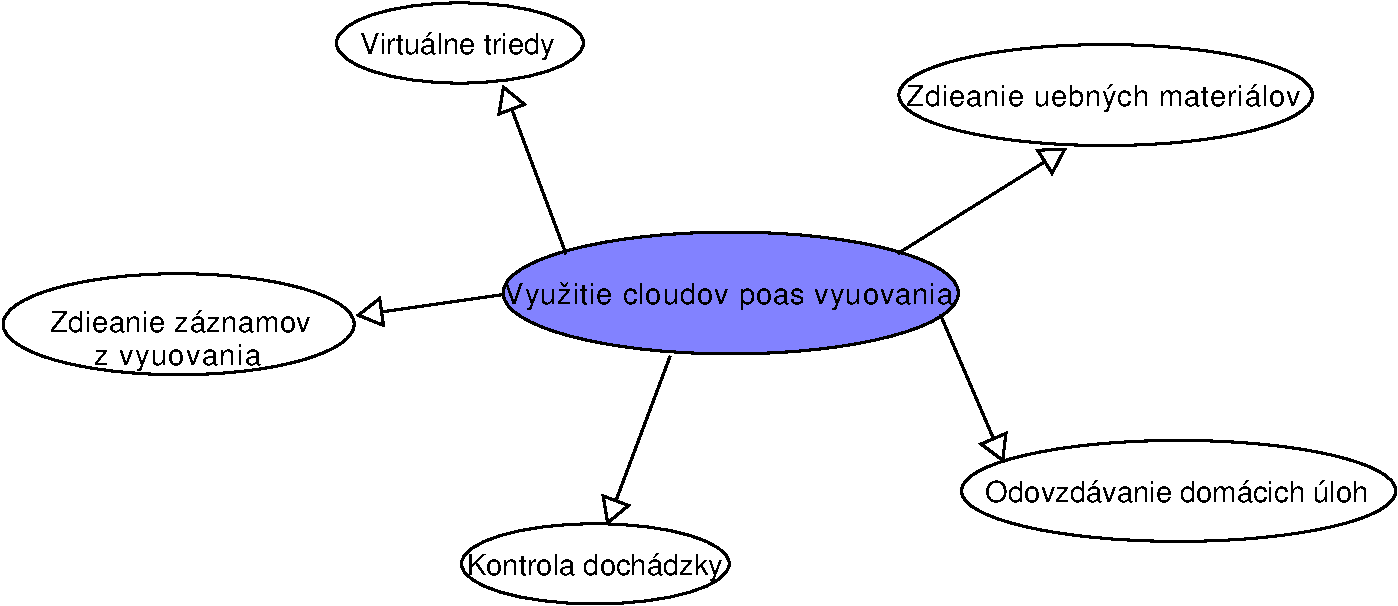
\includegraphics[width=1\textwidth]{Obrázky/opis-crop.pdf}
%\caption{Prvý diagram}
%\end{figure}


% týmto sa generuje zoznam literatúry z obsahu súboru literatura.bib podľa toho, na čo sa v článku odkazujete
\bibliography{literatura}
\bibliographystyle{plain} % prípadne alpha, abbrv alebo hociktorý iný
\end{document}
